% !TeX spellcheck = en_US

\chapter{Analysis}
This chapter is about identifying the requirements, needed to transform the application into a micro-service front-end.\\
The Analysis first determines use-cases for the system, based on the stakeholders. These use-cases will be converted into requirements, which are distinguished into functional and non-functional. A gap-analysis is finally performed, to compare requirements of the new system to the old implementation. 


\section{Stakeholders}
Stakeholders are groups of people with an interest in the system. This interest can be from a practical user based standpoint, as well as from a management standpoint.

\subsection{Model Developer}
The model developer is a technical user that creates a MARS model in cooperation with a domain expert. His main goal is to make sure the model, he created executes correctly and without errors.

\subsection{Simulation Creator}
The simulation creator is a domain expert. He uses the model, created by the model developer to answer a research question. The model developer does that by running various simulations with a given model. He adjusts the parameters of the scenario, in order to determine their impact on the result and to prove or to disprove his theories.

\subsection{Group Administrator}
The Group Admin is a user of the system with a leading roll in his group. He wants to manage people belonging to a particular group and handle group dependent settings. He also wants to add users to his group, remove them and handle permissions for data, owned by his group.

\subsection{Administrator}
The Administrator is a global user with far reaching permission inside the system. An admin is able to alter any kind of data inside the system. He holds global responsibility and is the only one, who is capable of activating new users.


\section{Use-cases}
The workflow that includes completing all the necessary steps to start a simulation can be broken down into five parts: \textit{Import Data}, \textit{Check imported Files}, \textit{Create Mapping}, \textit{Start Simulation} and \textit{View Results} (see section \ref{sec:workflow}). This piece of work does not cover the whole workflow. Instead, it is focused on the first three use-cases.\\
The Use-cases \textit{Manage Groups} and \textit{Manage Users} are for administrative purposes only. They are also not in the scope of this paper.\\
Figure \ref{fig:use-cases} shows an overview of the mentioned use-cases with their stakeholders. Note, that although the Model Developer and the Simulation Creator have a different view of the system, their use-cases do not differ. This is why future sections will reference them as users.
\begin{figure}[H]
	\centering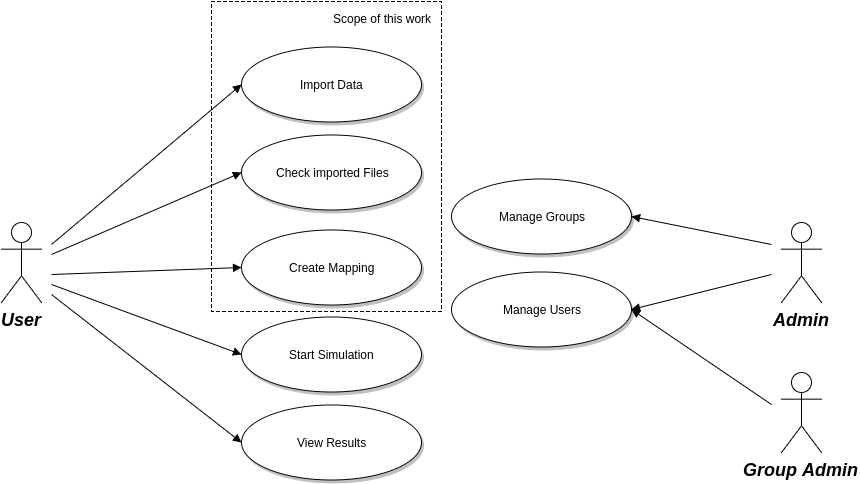
\includegraphics[width=1\textwidth]{res/Use-Cases_reduced}
	\caption{Use-cases for the Websuite}
	\label{fig:use-cases}
\end{figure}

\subsection{Import Files}
\begin{usecase}
	\addtitle{Import I}{Data}
	\addfield{Summary:}{Upload local data files to the Websuite, to use them for a simulation. The following data types have to be supported: 
	\begin{itemize}
		\item Geo-potential-field data (.csv)
		\item Grid-potential-field data (.csv)
		\item Obstacle-layer data (.csv)
		\item Table-based data (.csv)
		\item Time-series data (.csv)
		\item GIS data (.asc, .tif, .shp)
	\end{itemize}
	}
	\additemizedfield{Actors:}{
		\item User
	}
	\additemizedfield{Preconditions:}{
		\item \textit{Import Data} page is open.
	}
	\additemizedfield{Primary Scenario:}{
		\item The user drags one or multiple files onto the upload window, fills the form for every file and starts the import.
	}
	\additemizedfield{Alternative Scenario:}{
		\item The user clicks the upload button, browses files of his local machine, fills the form for every file and starts the import.
	}
\end{usecase}

\begin{usecase}
	\addtitle{Import II}{Model}
	\addfield{Summary:}{Upload local model files to the Websuite, to use them for a mapping.}
	\additemizedfield{Actors:}{
		\item User
	}
	\additemizedfield{Preconditions:}{
		\item \textit{Import Model} page is open.
	}
	\additemizedfield{Primary Scenario:}{
	\item The user drags one or multiple files onto the upload window, fills the form for every file and starts the import.
	}
	\additemizedfield{Alternative Scenario:}{
		\item The user clicks the upload button, browses files of his local machine, fills the form for every file and starts the import.
	}
\end{usecase}

\begin{usecase}
	\addtitle{Import III}{Bulk}
	\addfield{Summary:}{Upload multible files to the Websuite, with the same metadata, to save time for files that are handled alike.}
	\additemizedfield{Actors:}{
		\item User
	}
	\additemizedfield{Preconditions:}{
		\item \textit{Import Data} page is open.
	}
	\additemizedfield{Primary Scenario:}{
		\item The user drags one or multiple files onto the upload window, fills the one form and starts the import.
	}
	\additemizedfield{Alternative Scenario:}{
		\item The user clicks the upload button, browses files of his local machine, fills the one form and starts the import.
	}
\end{usecase}

\subsection{Check imported Files}
\begin{usecase}
	\addtitle{View I}{Search \& filter results}
	\addfield{Summary:}{Find specific input data with the help of a search and filter functionality.}
	\additemizedfield{Actors:}{
		\item User
	}
	\additemizedfield{Preconditions:}{
		\item \textit{Data View} page is open
		\item Files have been imported
	}
	\additemizedfield{Primary Scenario:}{
		\item The user views imported files, filters them by category and sorts them by name.
	}
	\additemizedfield{Alternative Scenario:}{
		\item The user filters by text input and sorts them by category.
	}
\end{usecase}

\begin{usecase}
	\addtitle{View II}{Check processing result}
	\addfield{Summary:}{Make sure all the imported files from data- and modelimport were processed correctly.}
	\additemizedfield{Actors:}{
		\item User
	}
	\additemizedfield{Preconditions:}{
		\item \textit{Data View} page is open
		\item Files have been imported
	}
	\additemizedfield{Primary Scenario:}{
		\item The user checks the status of multible imported files by searching for them. As a result he sees \textit{Finished} or \textit{Failed}.
	}
\end{usecase}

\begin{usecase}
	\addtitle{View III}{View metadata:}
	\addfield{Summary:}{View the metadata of a specific imported file.}
	\additemizedfield{Actors:}{
		\item User
	}
	\additemizedfield{Preconditions:}{
		\item \textit{Data View} page is open
		\item Files have been imported
	}
	\additemizedfield{Primary Scenario:}{
		\item The user clicks on a specific import entry and views the metadata inside a modal window.
	}
\end{usecase}

\subsection{Scenarios}
\begin{usecase}
	\addtitle{Scenario I}{Create new scenario}
	\addfield{Summary:}{Create a scenario based on a model.}
	\additemizedfield{Actors:}{
		\item User
	}
	\additemizedfield{Preconditions:}{
		\item \textit{Create Scenario} page is open
		\item A model has been uploaded.
	}
	\additemizedfield{Primary Scenario:}{
		\item The user clicks the "add Scenario" button. Inside the new modal, he specifies a name, selects a model and saves the new scenario.
	}
\end{usecase}

\begin{usecase}
	\addtitle{Scenario II}{Create scenario as copy}
	\addfield{Summary:}{Create a scenario based on an existing scenario. This clones the original scenario with all its mapping and saves it under a different name.}
	\additemizedfield{Actors:}{
		\item User
	}
	\additemizedfield{Preconditions:}{
		\item \textit{Create Scenario} page is open
		\item A model has been uploaded.
		\item At least one scenario exists.
	}
	\additemizedfield{Primary Scenario:}{
		\item The user clicks the "clone Scenario" button. Inside the new modal, he changes the name and description and saves the new scenario.
	}
\end{usecase}

\begin{usecase}
	\addtitle{Scenario III}{Create Mapping}
	\addfield{Summary:}{Combine the fields from the uploaded model with uploaded data.}
	\additemizedfield{Actors}{
		\item User
	}
	\additemizedfield{Preconditions:}{
		\item \textit{Create Mapping} page is open
		\item Data has been imported.
		\item A Model has been imported.
		\item A scenario has been selected.
	}
	\additemizedfield{Primary Scenario:}{
		\item The user connects the required fields to a dataset. He then sets the global parameters for the simulation.
	}
\end{usecase}



\section{Requirements}
\label{sec:requirements}
Derived from the use-cases, the following requirements have been created.


\subsection{Functional Requirements}

\subsubsection{Import}
\reqstartF
\item The WebUI has a component that is capable of importing data files for the simulation (data import).
\item The data import supports the \textit{Geo-potential-field} data type.
\item The data import supports the \textit{Grid-potential-field} data type.
\item The data import supports the \textit{Obstacle-layer} data type.
\item The data import supports the \textit{Table-based} data type.
\item The data import supports the \textit{Time-series} data type.
\item The data import supports the \textit{GIS} data type.
\item The data import supports uploading multiple files with the same metadata (bulk upload).
\item The WebUI has a component that is capable of importing model files for the simulation (model import).
\item The imports support drag and drop for file selection.
\item The imports support browsing the local computer for file selection.
\item Both imports show the processing of the uploaded files in a view, that is displayed independently of the import page.
\reqendF

\subsubsection{View}
\reqstartF
\item The WebUI has a component which allows the user to view the metadata of uploaded files (data view).
\item The data view allows reordering the displayed files.
\item The data view supports filtering the displayed files via text input.
\item The data view supports filtering the displayed files by data type, import status and tag.
\item The data view supports pagination of the displayed data.
\reqendF

\subsubsection{Scenario}
\reqstartF
\item The WebUI has a component that allows creating scenarios based on an imported model (Scenario view).
\item The scenario view allows the user to display the already created scenarios.
\item The scenario view allows the user to change the name of a scenario.
\item The scenario view supports duplicating a scenario.
\item Scenarios can be selected from every page.
\reqendF

\subsubsection{Mapping}
\reqstartF
\item The WebUI has a component which allows the user to connect uploaded data files to a scenario (mapping view).
\item The mapping view supports transferring multiple mappings of one file to another one.
\item The mapping can be created manually by the user.
\item The mapping view filters the available data files, so only compatible files are shown.
\item The mapping view lets the the user filter compatible mappings by name and tag.
\item When a mapping is created, the next available field is automatically selected.
\item The mapping view renders the correct input type depending on the allowed value (e.g. date-picker for date, checkbox for boolean, etc.).
\item The mapping view shows the validation result from the back-end, once a mapping has been saved.
\item The mapping view supports mapping of global parameters.
\item Global scenario parameters can be added and removed by the user.
\reqendF


\subsection{Non-Functional Requirements}
\reqstartNF
\item Input fields for all components only allow the required type of input.
\item The data import and model import share one code base (no duplicate code).
\item Adding new supported data types can be done in one central place.
\item The WebUI does not rely on the existence of other services.
\item Errors have to be communicated to the user.
\item The application works in every browser that supports HTML5.
\item No additional software installation is required on the client side.
\item The WebUI can be deployed into a Kubernetes cluster.
\reqendNF



\section{Gap-Analysis}
The following table shows the difference between the old Websuite, compared to the requirements from the previous chapter.

\begin{table}[H]
	\caption{Comparison of the old Websuite and the new requirements.}
	\begin{tabularx}{\textwidth}{|X|l|l|}
	\hline
	\textbf{Feature} & \textbf{old Websuite} & \textbf{WebUI} \\ \hline
	The data import supports the \textit{Geo-potential-field} data type. & no & yes \\ \hline
	The data import supports the \textit{Grid-potential-field} data type. & no & yes \\ \hline
	The data import supports the \textit{Obstacle-layer} data type. & no & yes \\ \hline
	The data import supports uploading multiple files with the same metadata (bulk upload). & no & yes \\ \hline
	Both imports show the processing of the uploaded files in a view, that is displayed independently of the import page. & no & yes \\ \hline
	The mapping view filters the available data files, so only compatible files are shown. & no & yes \\ \hline
	The scenario view supports duplicating a scenario. & no & planned \\ \hline
	Scenarios can be selected from every page. & no & yes \\ \hline
	The mapping view supports transferring multiple mappings of one file to another one. & no & yes \\ \hline
	The mapping view filters the available data files, so only compatible files are shown. & no & yes \\ \hline
	The mapping view lets the the user filter compatible mappings by name and tag. & no & planned \\ \hline
	The mapping view renders the correct input type depending on the allowed value & doesn't apply & yes \\ \hline
	The mapping view shows the validation result from the back-end, once a mapping has been saved. & no & yes \\ \hline
	Input fields for all components only allow the required type of input. & no & yes \\ \hline
	The data import and model import share one code base (no duplicate code). & no & yes \\ \hline
	Adding new supported data types can be done in one central place. & no & planned \\ \hline
	The WebUI does not rely on the existence of other services. & no & yes \\ \hline
	The WebUI can be deployed into a Kubernetes cluster. & no & yes \\ \hline
	\end{tabularx}
\end{table}
